\section{LSM9DS1}
Der benyttes et integrated circuit (IC) af typen LSM9DS1, som både indeholder magnometer, gyroskop og accelerometer, hvoraf magnometret ikke benyttes. Det er muligt at indstille accelerometeret til $\pm$1, $\pm$4, $\pm$8 eller $\pm$16 g, og gyroskopet kan indstilles til $\pm$245, $\pm$500 eller $\pm$2000 grader per sekund. \citep{Jimb02016} \newline
LSM9DS1 har ni frihedsgrader, hvilket betyder, at den måler i x-, y- og z-aksen for både magnometret, gyroskopet og accelerometeret, som kan ses på \figref{vores_IC}. %Akserne for gyroskopet og accelerometeret internt følger højrehåndsreglen.
\citep{Jimb02016}\newline 
\begin{figure}[H]
	\centering
	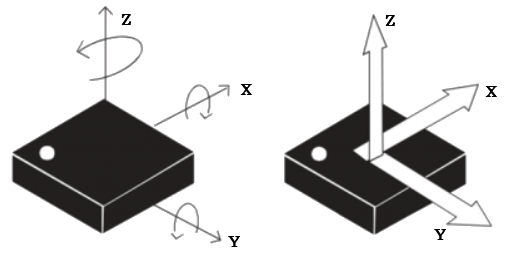
\includegraphics[scale=0.6]{figures/cDesign/LSM9DS1.png}
	\caption{På figuren ses akserne fra LSM9DS1. Til venstre ses magnometret, hvis akser er drejet én omgang i forhold til de to andre sensorer. I midten ses gyroskopet med sine roterende akser og til højre ses accelerometerets akser.\citep{Jimb02016}}
	\label{vores_IC}
\end{figure}
Accelerometeret kan både bruges med en SPI og en I$^{2}$C styrefunktion, og mikrokontrolleren besidder begge. Der ønskes at benytte I$^{2}$C funktionen, da IC'en både skal sende og modtage data.\fxnote{Modtage om gyroskopet skal tændes eller slukkes.} For at benytte I$^{2}$C funktionen sættes pin CS\_AG høj, og de fire pins SDO og CS benyttes ikke. Alle pins kan ses på \figref{IC_pins}
\begin{figure}[H]
	\centering
	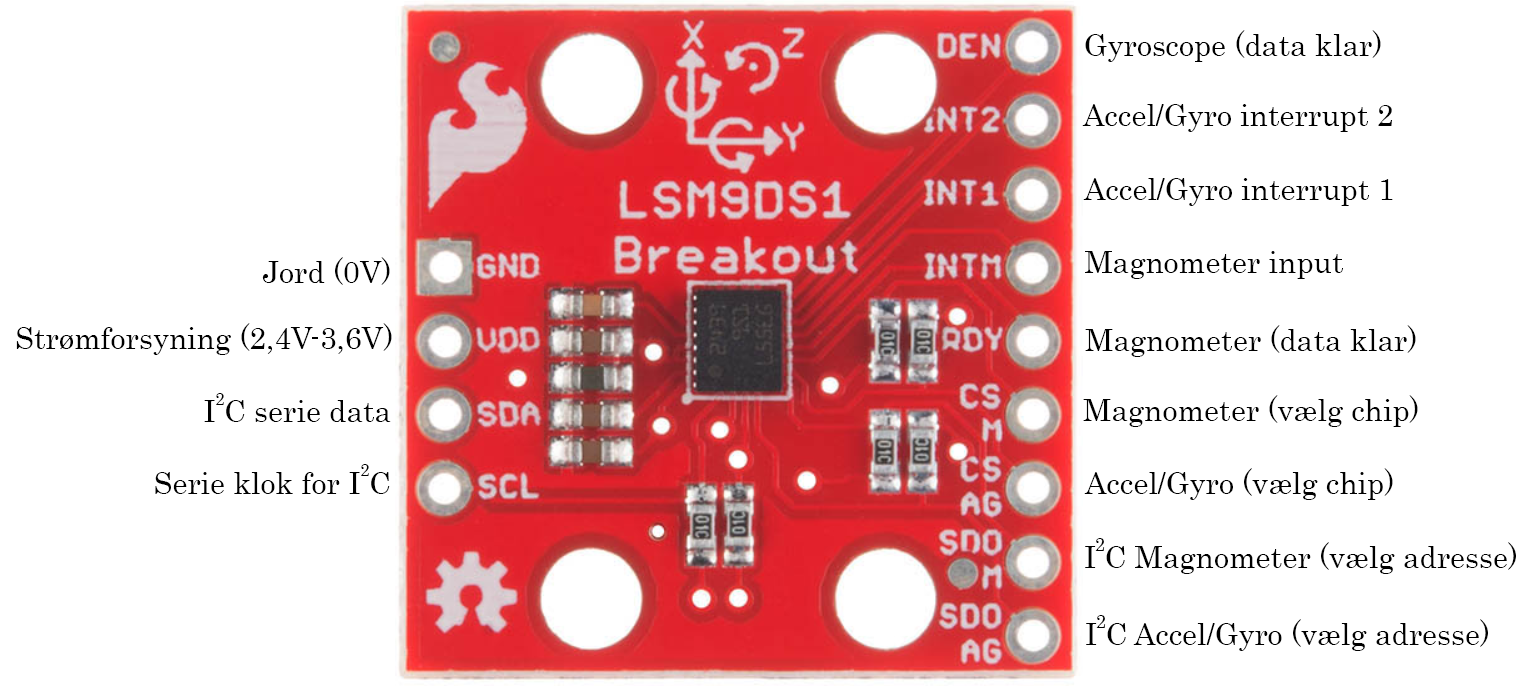
\includegraphics[scale=0.35]{figures/cDesign/accelerometeret.png}
	\caption{På figuren ses udgangene fra IC'en.\citep{Jimb02016}}
	\label{IC_pins}
\end{figure}
I LSM9DS1 bruger gyroskopet 4 mA og accelerometeret bruger 600$\mu$ A. Det er derfor væsentligt, at gyroskopet bruges minimalt, når systemet skal være batteridrevet. Det er muligt enten at slukke begge sensorer, at benytte accelerometeret alene eller benytte både accelerometeret og gyroskopet sammen, hvor de har samme mængde output af data. Der kan yderligere spares strøm ved brug af gyroskopet, hvis der vælges en lavere samplerate. % alt efter hvor hurtigt et signal skal samples. 
Gyroskopet har tre forskellige power modes: slukket, low power og normal power. For at gyroskopet kan være i low power, skal outputtet af data være på 14,9-119 Hz. Hvis outputsignalet er over dette, vil gyroskopet automatisk gå i normal power. 
